\newpage

\section{Bestimmtes Integral}

\subsection{Definition Integral}
Gegeben ist eine auf dem Intervall $[a,b]$ stetige Funktion $f$. Wir unterteilen das Intervall $[a,b]$ in $n$ Teilintervalle $I_k$ der Länge $\Delta x = \frac{b-a}{n}$. In jedem Teilintervall $I_k$ wählen wir eine Stelle $x_k$. Der Wert, zu dem
\[
    \sum_{k=1}^{n} f(x_k) \cdot \Delta x
\]
für ein immer grösser werdendes $n$ tendiert, heisst: bestimmtes Integral von $a$ bis $b$ über $f(x)$.
\[
    \int_{a}^{b} f(x)dx
\]

\begin{enumerate}
    \item $\int_{a}^{a} f(x) dx = 0$
    \item Gegeben $b < a$. Dann gilt: $\int_{a}^{b} f(x) dx = - \int_{a}^{b} f(x) dx$
    \item Gegeben ist $b \in [a, c]$. Dann gilt: $\int_{a}^{c} f(x) dx = \int_{a}^{b} f(x) dx + \int_{b}^{c} f(x) dx$
\end{enumerate}

\subsection{Stammfunktion}
Eine Stammfunktion von $f$ ist eine Funktion $F$, für die gilt:
\[
    F'(x) = f(x) \hspace{5em} \text{für alle } x \in I
\]

Gegeben sind zwei Stammfunktionen $F_1$ und $F_2$ einer Funktion $f$. Dann gibt es eine Konstante $c$, so dass gilt:
\[
    F_2(x) = F_1(x) + c \hspace{5em} \text{für alle } x
\]

\subsubsection{Hauptsatz der Differential- und Integralrechnung}
Gegeben ist eine Funktion $f$, die auf einem Intervall $I$ stetig ist, und eine beliebige Stammfunktion $F$ von $f$. Dann gilt für alle $a,b \in I$:
\[
    \int_{a}^{b} f(x) dx = F(b) - F(a)
\]

\subsection{Integrationsregeln}
Gegeben sind zwei Funktionen $f$ und $g$ mit Stammfunktionen $F$ bzw. $G$ sowie eine Konstante $c$. Dann gilt:
\begin{enumerate}
    \item $c \cdot F(x)$ ist eine Stammfunktion von $c \cdot f(x)$
    \item $F(x) + G(x)$ ist eine Stammfunktion von $f(x) + g(x)$
\end{enumerate}

Die Anwendung der obenstehenden Integrationsregeln zusammen mit dem Hauptsatz der Integralrechnung ergibt

\begin{enumerate}
    \item $\int_{a}^{b} c \cdot f(x) dx = c \cdot \int_{a}^{b} f(x) dx$
    \item $\int_{a}^{b}(f(x) + g(x)) dx = \int_{a}^{b} f(x) dx + \int_{a}^{b} g(x) dx$
\end{enumerate}

\vfill

\subsection{Integration von Polynomfunktionen}
Stammfunktion von $f(x) = c$ \\
$F(x)=c\cdot x$ \\
\\
Stammfunktion von $f(x) = x^n (n \in \mathbb{R}, n \neq -1)$ \\
$F(x)=\frac{1}{n+1} \cdot x^{n+1}$ \\
\\
Stammfunktion von $g(x) = \frac{1}{x}$ \\
$G(x) = \ln(|x|)$ \\
\\
\textbf{Beispiel: } $f(x) = 2x^2 + 3x -1$. Gesucht: $\int_{1}^{2} (2x^2 + 3x -1) dx$
\begin{align*}
    &\text{Stammfunktion von } 2x^2 + 3x -1: \\
    & F(x) = 2 \cdot (\frac{1}{3}x^3) + 3 \cdot (\frac{x^2}{2}) - x = \frac{2}{3}x^3 + \frac{3}{2}x^2 - 2 \\
    & \int_{1}^{2} f(x) dx = [F(x)]_1^2 = F(2)- F(1) = \frac{49}{6}
\end{align*}

\begin{center}
    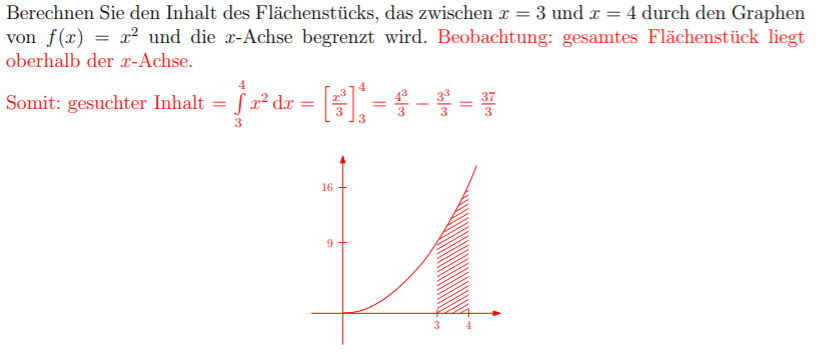
\includegraphics[width=1\linewidth]{images/integrationbsp.png}
\end{center}

\subsection{Ableitungen und Integrale ausgewählter Funktionen}
\subsubsection{Potenz- und Logarithmus-Funktionen}
\begin{enumerate}
    \item $\int a^x dx = \frac{a^x}{\ln(a)} + C$
    \item $\int \ln(x) dx = x \cdot \ln(x) - x + C$
    \item $\int \log_a (x)dx = \frac{1}{\ln(a)}\cdot (x \cdot \ln(x) - x) + C$
\end{enumerate}

\subsubsection{Trigonometrische Funktionen}
\begin{itemize}
    \item $\int \sin (x) dx = - \cos (x) + C$
    \item $\int \cos (x) dx = \sin (x) + C$
    \item $\int \tan (x) dx = - \ln |\cos (x) | + C$
    \item $(\tan(x))' = 1 + \tan^2(x) = \frac{1}{\cos^2(x)} \text{ resp. } \int(1+\tan^2(x)) dx = \int \frac{1}{\cos^2(x)} dx = \tan(x) + C$
    \item $(\arcsin (x))'= (1-x^2)^{-1/2} \text{ resp. } \int (1-x^2)^{-1/2}dx= \arcsin(x) + C$
    \item $(\arccos(x))' = -(1-x^2)^{-1/2} \text{ resp. } \int - (1 - x^2)^{-1/2} dx = \arccos(x) + C$
    \item $(arctan(x))' = (1 + x^2)^{-1} \text{ resp. } \int (1 + x^2)^{-1} dx = \arctan(x) + C$
\end{itemize}

